\documentclass[11pt, a4paper]{article}

\usepackage{graphicx}

\begin{document}

\title{\textbf{Documentation}\\ Rust and CakeML Communication via the Prosper Hypervisor}
\maketitle

\pagebreak

\section*{System Specification, Motivation and Attacker Model}
The system consists of three components: The Prosper hypervisor and two guests.
The hypervisor has been formally verified to isolate the CPU to only depend on
and affect the guest that the CPU is executing. The hypervisor configures the
page tables such that in unprivileged mode, the CPU can only access the memory
allocated to the guest the CPU is currently executing. The page tables are
located in Linux memory but are configured such that Linux cannot modify the
page tables. The guests can only communicate via channel provided by the
hypervisor based on input and output buffers of the guests.

In addition to the CPU, the network interface controller (NIC) can also access
memory. The page tables are configured such that Linux can only read DMA
registers, and if Linux attempts to write them, an exception is raised, causing
the hypervisor to be invoked, which invokes a NIC monitor. The monitor checks
that the attempted DMA register write cannot cause the NIC to access non-Linux
memory nor modify the page tables. Regarding formal verification of NIC
isolation, isolating conditions of the NIC have been formally verified, and that
the transmission part of the monitor respects the verified isolation conditions.

By letting Linux be one guest, and a critical application be the other guest
(e.g. CakeML), this system allows a feature rich untrusted software component
(e.g. Linux) to interact in a controlled manner with a critical guest, without
corrupting that guest. For instance, Linux can provide Internet access via its
TCP/IP stack and Ethernet driver, and USB storage via its file system and USB
infrastructure, which is probably many tens of thousands of lines of code,
without enabling this code to directly affect the critical application.

The attacker model is thus a Linux guest that is completely untrusted and upon
which no assumptions are made.

\section*{Software Interaction}
The Prosper hypervisor provides isolation between itself and two guests. One
guest is a paravirtualized (modified/ported) Linux 5.15.13, and the other is a
CakeML application. A rust application is running in Linux, and communicates
with the CakeML guest via a communication channel provided by the hypervisor.

\begin{figure}
\center
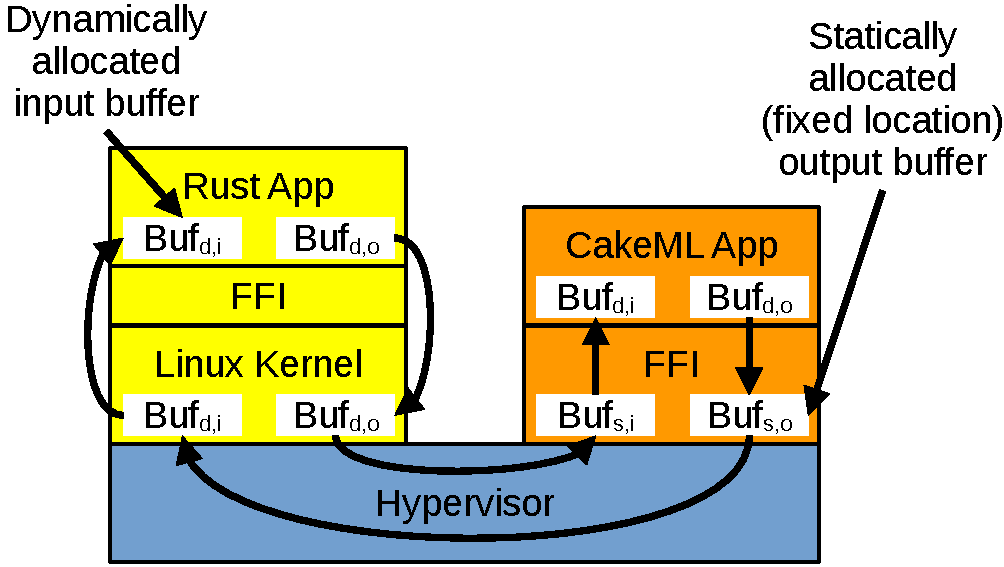
\includegraphics[scale=0.7]{overview}
\caption{Rust and CakeML interaction through the hypervisor.}
\label{fig:overview}
\end{figure}

A step-based description of the guest communication is as follows (see
Figure~\ref{fig:overview}):
\begin{enumerate}
\item
	Rust allocates "dynamic" input and output buffers, and stores data in the
	output buffer.
\item
	Rust invokes the FFI, which issues a system call to Linux, specifying the
	locations of the buffers and their size.
\item
	The Linux system call allocates kernel buffers, and copies the data in the
	dynamic Rust output buffer to a Linux kernel output buffer, and invokes the
	hypervisor.
\item
	The hypervisor copies the data from the Linux kernel output buffer to a
	fixed located input buffer of CakeML, and transfers control to CakeML.
\item
	The CakeML FFI transfers the data in the fixed CakeML buffer to a
	dynamically allocated CakeML buffer in the CakeML application.
\item
	CakeML processes the received data and stores the result in a dynamically
	allocated output buffer and invokes the FFI.
\item
	The CakeML FFI transfers the data in the dynamically allocated output buffer
	to the fixed located output buffer and invokes the hypervisor.
\item
	The hypervisor copies the data in the fixed located output buffer of CakeML
	to the input buffer of the Linux kernel, and transfers control to the Linux
	system call.
\item
	The Linux system call copies the data from the kernel input buffer to the
	Rust input buffer, and returns to Rust.
\item
	Rust processes the received data, and the communication cycle goes back to
	step 1.
\end{enumerate}

The Rust application invokes the hypervisor by means of a foreign function
interface written in C:
\\
\\\textit{invoke\_cake}(\textit{output\_buffer}, \textit{output\_buffer\_size}, \textit{input\_buffer}, \textit{input\_buffer\_size}).
\\\\
This function takes addresses and sizes of input and output buffers of the Rust
application, and performs a system call to Linux. The system call in Linux first
allocates Linux kernel input and output buffers, then copies the data of the
Rust application output buffer to the Linux kernel output buffer, and third
invokes a hypercall of the hypervisor with the physical addresses and sizes as
arguments.

The reason for having Linux kernel buffers in addition to the Rust application
buffers is to enable the hypervisor to identify the physical addresses of the
buffers (using a simple virtual address offset \texttt{0xC0000000} to convert virtual
addresses to physical addresses and vice versa), in contrast to Linux
application buffers that can be at arbitrary locations in memory.

The hypervisor checks that the identified Linux kernel buffer locations are
allocated to Linux (and not the hypervisor or CakeML, to preserve isolation;
see hypervisor//core//hypervisor//handlers.c). Otherwise, the communication is
blocked (an error message is printed and the system freezes). If the buffers are
in Linux allocated memory, the hypervisor copies the data in the Linux kernel
output buffer to the CakeML input buffer (at the fixed virtual address
\texttt{0xF0F00000} allocated to the CakeML guest; see
hypervisor/core/hw/board/beaglebone/board\_mem.c). The hypervisor then invokes
CakeML (whose program counter is initialized in
hypervisor/core/hypervisor/guest\_config/linux\_config.c by the macro \texttt{TRUSTED\_RPC};
see hypervisor-cakeml//cakeml//start.S, where \texttt{TRUSTED\_RPC} is set to the 6th 4-byte
word because the first instruction in start.S is a nop being skipped and the
following 5 words are for the size of the buffers, at the moment 4 bytes times
5 words = 20 bytes).

CakeML continues (or starts) its execution, which (if everything goes to plan)
copies the data via a foreign function interface from the fixed input buffer to
a buffer dynamically allocated by CakeML. CakeML then processes the data and
then via another foreign function interface copies the data of dynamically
allocated buffer of CakeML to a fixed output buffer location, and invokes the
hypervisor. The hypervisor copies the data in the fixed output buffer location
to the Linux kernel input buffer, and invokes Linux.

The Linux system call copies the data in the Linux kernel input buffer to the
Rust application input buffer, and returns to the Rust application.

\section*{Hypervisor Changes}
The Rust application triggered execution of some Linux kernel code that causes
alignment faults (addressing a memory location whose address is not a multiple
of 4). This type of fault causes a data abort exception. Such exceptions were
analyzed by the previous version of the hypervisor to check whether they were
caused by Linux attempting to write an executable page (the DMMU component of
the hypervisor enforces the W XOR X policy to ensure that only trusted software
is executed; however, at the moment there is no mechanism checking that
executable pages satisfy a certain trusted property). This analysis ignored the
possibility of alignment faults (which have nothing to do with access permission
violations), and the system crashed. The updated version of the hypervisor
forwards data abort exceptions due to alignment faults directly to Linux, which
handles them as intended.

\section*{Linux Changes}
The Rust application is linked by the Rust compiler with precompiled libraries
that contain thumb code. This code caused undfined instruction exceptions, which
the hypervisor forwards to Linux. This type of exception caused the exception
handler of the previous paravirtualized Linux kernel to access uninitialized
data structures (since they are not intended to be used by Linux when executed
on top of the hypervisor) and perform privileged operations (which can only be
performed by the hypervisor, and which in this case are not supported). The
Linux code associated with these operations is excluded from compilation by
means of a macro.

\section*{Compilation for BBB}
The following summarizes the compilation steps for running the software on
BeagleBone Black. Detailed instructions are listed in the text file 'Installation and run instructions.txt'.

\begin{enumerate}
\item
	Compile the rust application statically (in order to avoid dependence on
	dynamically linked libraries; invoke\_cakeml.c implements the foreign
	function interface):

		\textbf{cd \textless path to cakeml-kth-repo\textgreater/cakeml-kth-repo/hypervisor-cakeml/linuxapp/}
\\\\
		\textbf{\textless path to buildroot-2021.02.8\textgreater/buildroot-2021.02.8/output/host/usr/bin/arm-buildroot-linux-gnueabihf-gcc-8.4.0 -static -c invoke\_cakeml.c -o invoke\_cakeml.o}
\\\\
		\textbf{\textless path to buildroot-2021.02.8\textgreater/buildroot-2021.02.8/output/host/usr/bin/arm-buildroot-linux-gnueabihf-ar rcs libinvoke\_cakeml.a invoke\_cakeml.o}
\\\\
		\textbf{\textless path to buildroot-2021.02.8\textgreater/buildroot-2021.02.8/output/host/usr/bin/rustc --target=armv7-unknown-linux-gnueabihf -Clinker=arm-linux-gnueabihf-gcc -Ctarget-feature=+crt-static -L . rust\_app.rs -o rust\_app}
\item
	Update the filesystem used by Linux by placing the compiled rust
	application, rust\_app, in the root (home directory of the user root)
	directory:

		\textbf{cd \textless path to buildroot-2021.02.8\textgreater/buildroot-2021.02.8/output/images}
\\\\
		\textbf{sudo rm -rf rootfs}
\\\\
		\textbf{mkdir rootfs}
\\\\
		\textbf{cd rootfs}
\\\\
		\textbf{sudo cpio -i -d -H newc -F ../rootfs.cpio --no-absolute-filenames}
\\\\
		\textbf{cd ..}
\\\\
		\textbf{sudo chown root rootfs -R}
\\\\
		\textbf{sudo cp ../../../cakeml-kth-repo/hypervisor-cakeml/linuxapp/rust\_app ./rootfs/root/rust\_app}
\item
	Compile Linux and copy the binary exeutable image to the linux guest directory of the hypervisor:

		\textbf{cd \textless path to linux-5.15.1\textgreater}
\\\\
		\textbf{make ARCH=arm CROSS\_COMPILE=arm-linux-gnueabihf- -j8}
\\\\
		\textbf{cd ..}
\\\\
		\textbf{cat linux-5.15.13/arch/arm/boot/zImage linux-5.15.13/arch/arm/boot/dts/am335x-boneblack.dtb \textgreater hypervisor/guests/linux/build/zImage.bin}

\item
	Compile the CakeML guest and copy the binary executable image to trusted
	guest directory of the hypervisor (trusted.S is the binary CakeML code,
	basis\_ffi.c is the implementation of the foreign function interface, print.c
	contains routines for printing to the terminal for debugging, start.S
	contains the declaration of the fixed located input and output buffers of
	CakeML and the entry code of CakeML):

		\textbf{\textless path to CakeML compiler\textgreater/cake --target=arm7  <trusted.cml >trusted.S -B}
\\\\
		\textbf{arm-none-eabi-gcc -nostdlib trusted.S basis\_ffi.c print.c start.S -T cake\_guest.ld -o trusted}
\\\\
		\textbf{arm-none-eabi-objcopy trusted -O binary trusted.bin}
\\\\
		\textbf{cp trusted.bin \textless path to hypervisor\textgreater/hypervisor/guests/trusted/build/trusted.bin}
\item
	Start docker and compile the hypervisor:

		\textbf{cd \textless path to source directory of the hypervisor\textgreater}
\\\\
		\textbf{sudo docker run --rm -v "\$PWD":/usr/src/myapp -w /usr/src/myapp -it gcc49-arm-docker}
\\\\
		\textbf{make}
\item
	Run on BeagleBone Black.
\end{enumerate}

\section*{Compilation for x86}
Invoke the script compile\_hypervisor\_emulation.sh. It first compiles the CakeML
application by defining the macro \texttt{EMULATE\_HYPERVISOR} (used for basis\_ffi.c). It
then compiles the Rust application by creating a C library invoke\_cakeml.c by
defining the macro \texttt{EMULATE\_HYPERVISOR}, and then the Rust code with the Rust
configuration macro \texttt{emulate\_hypervisor}. Finally it compiles emulation.c, which
sets up the pipes and creates a child process, with the parent being replaced
with the CakeML application and the child being replaces by the Rust
application.

\end{document}